% Options for packages loaded elsewhere
\PassOptionsToPackage{unicode}{hyperref}
\PassOptionsToPackage{hyphens}{url}
\documentclass[
]{article}
\usepackage{xcolor}
\usepackage[margin=1in]{geometry}
\usepackage{amsmath,amssymb}
\setcounter{secnumdepth}{-\maxdimen} % remove section numbering
\usepackage{iftex}
\ifPDFTeX
  \usepackage[T1]{fontenc}
  \usepackage[utf8]{inputenc}
  \usepackage{textcomp} % provide euro and other symbols
\else % if luatex or xetex
  \usepackage{unicode-math} % this also loads fontspec
  \defaultfontfeatures{Scale=MatchLowercase}
  \defaultfontfeatures[\rmfamily]{Ligatures=TeX,Scale=1}
\fi
\usepackage{lmodern}
\ifPDFTeX\else
  % xetex/luatex font selection
\fi
% Use upquote if available, for straight quotes in verbatim environments
\IfFileExists{upquote.sty}{\usepackage{upquote}}{}
\IfFileExists{microtype.sty}{% use microtype if available
  \usepackage[]{microtype}
  \UseMicrotypeSet[protrusion]{basicmath} % disable protrusion for tt fonts
}{}
\makeatletter
\@ifundefined{KOMAClassName}{% if non-KOMA class
  \IfFileExists{parskip.sty}{%
    \usepackage{parskip}
  }{% else
    \setlength{\parindent}{0pt}
    \setlength{\parskip}{6pt plus 2pt minus 1pt}}
}{% if KOMA class
  \KOMAoptions{parskip=half}}
\makeatother
\usepackage{graphicx}
\makeatletter
\newsavebox\pandoc@box
\newcommand*\pandocbounded[1]{% scales image to fit in text height/width
  \sbox\pandoc@box{#1}%
  \Gscale@div\@tempa{\textheight}{\dimexpr\ht\pandoc@box+\dp\pandoc@box\relax}%
  \Gscale@div\@tempb{\linewidth}{\wd\pandoc@box}%
  \ifdim\@tempb\p@<\@tempa\p@\let\@tempa\@tempb\fi% select the smaller of both
  \ifdim\@tempa\p@<\p@\scalebox{\@tempa}{\usebox\pandoc@box}%
  \else\usebox{\pandoc@box}%
  \fi%
}
% Set default figure placement to htbp
\def\fps@figure{htbp}
\makeatother
% definitions for citeproc citations
\NewDocumentCommand\citeproctext{}{}
\NewDocumentCommand\citeproc{mm}{%
  \begingroup\def\citeproctext{#2}\cite{#1}\endgroup}
\makeatletter
 % allow citations to break across lines
 \let\@cite@ofmt\@firstofone
 % avoid brackets around text for \cite:
 \def\@biblabel#1{}
 \def\@cite#1#2{{#1\if@tempswa , #2\fi}}
\makeatother
\newlength{\cslhangindent}
\setlength{\cslhangindent}{1.5em}
\newlength{\csllabelwidth}
\setlength{\csllabelwidth}{3em}
\newenvironment{CSLReferences}[2] % #1 hanging-indent, #2 entry-spacing
 {\begin{list}{}{%
  \setlength{\itemindent}{0pt}
  \setlength{\leftmargin}{0pt}
  \setlength{\parsep}{0pt}
  % turn on hanging indent if param 1 is 1
  \ifodd #1
   \setlength{\leftmargin}{\cslhangindent}
   \setlength{\itemindent}{-1\cslhangindent}
  \fi
  % set entry spacing
  \setlength{\itemsep}{#2\baselineskip}}}
 {\end{list}}
\usepackage{calc}
\newcommand{\CSLBlock}[1]{\hfill\break\parbox[t]{\linewidth}{\strut\ignorespaces#1\strut}}
\newcommand{\CSLLeftMargin}[1]{\parbox[t]{\csllabelwidth}{\strut#1\strut}}
\newcommand{\CSLRightInline}[1]{\parbox[t]{\linewidth - \csllabelwidth}{\strut#1\strut}}
\newcommand{\CSLIndent}[1]{\hspace{\cslhangindent}#1}
\setlength{\emergencystretch}{3em} % prevent overfull lines
\providecommand{\tightlist}{%
  \setlength{\itemsep}{0pt}\setlength{\parskip}{0pt}}
\usepackage{bookmark}
\IfFileExists{xurl.sty}{\usepackage{xurl}}{} % add URL line breaks if available
\urlstyle{same}
\hypersetup{
  pdftitle={Tree physiology},
  pdfauthor={Ivan Marbà Vologjanin},
  hidelinks,
  pdfcreator={LaTeX via pandoc}}

\title{Tree physiology}
\author{Ivan Marbà Vologjanin}
\date{2026-02-04}

\begin{document}
\maketitle

\subsection{Introduction}\label{introduction}

In recent decades, drought-driven tree mortality has become widespread,
particularly in \textbf{\emph{Mediterranean ecosystems}} (Lemus-Canovas
et al., 2024), where prolonged drought accelerates forest-to-shrubland
transitions (Coughlan de Perez et al., 2022). Detecting
\textbf{early-warning signals} of tree decline is therefore essential
for anticipating ecosystem changes and guiding conservation.

We investigated massive 2023 mortality event in Aleppo pine (\emph{Pinus
halepensis}) at the Garraf Massif (NE Iberian Peninsula).

\begin{figure}
\centering
\pandocbounded{\includegraphics[keepaspectratio]{images/location.JPEG}}
\caption{Mortality zone, Garraf 2024}
\end{figure}

This episode of drought-driven tree mortality from 2023 was reported in
the
\href{https://www.3cat.cat/3catinfo/boscos-que-moren-per-la-sequera-el-garraf-mes-a-prop-de-ser-un-paisatge-semidesertic/noticia/3276618/}{Catalan
news}. Despite the rains of recent months, the effects of the drought
remain
\href{https://www.3cat.cat/3catinfo/les-dues-cares-del-garraf-esplendor-per-les-pluges-pero-reducte-duna-sequera-persistent/noticia/3354963/}{visible}.

\section{Climatic data}\label{climatic-data}

Climatic data were obtained from the meteorological station at El Prat
Airport, which has recorded weather variables since 1950 (Prohom et al.,
2023). These are the trends of temperature and precipitation for the
period 1950-2022.

\pandocbounded{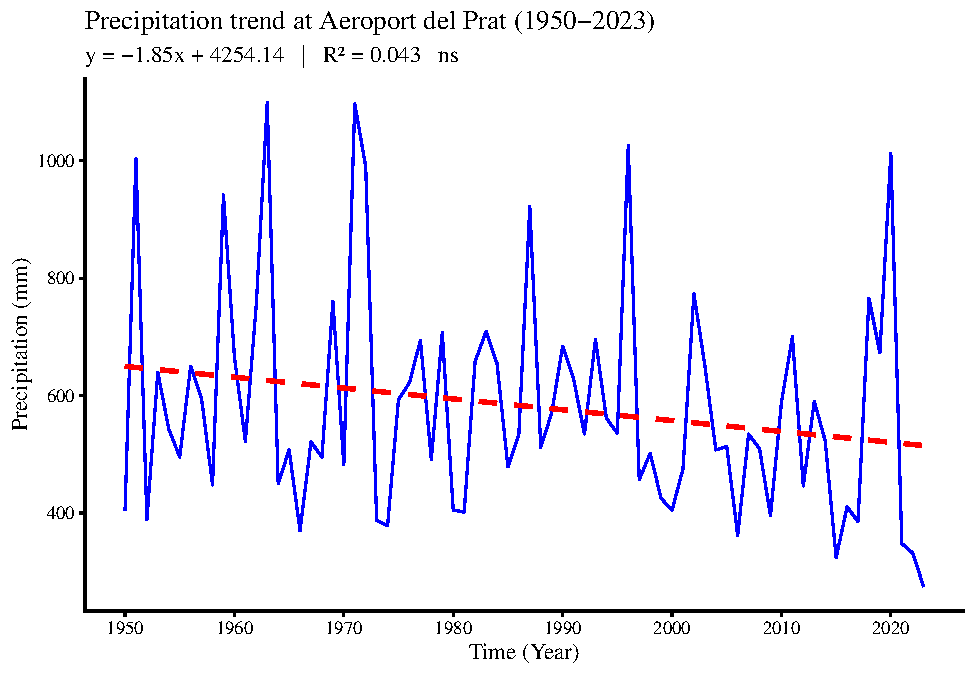
\includegraphics[keepaspectratio]{actividad2_4_files/figure-latex/unnamed-chunk-1-1.pdf}}

\section{DBH by status}\label{dbh-by-status}

\pandocbounded{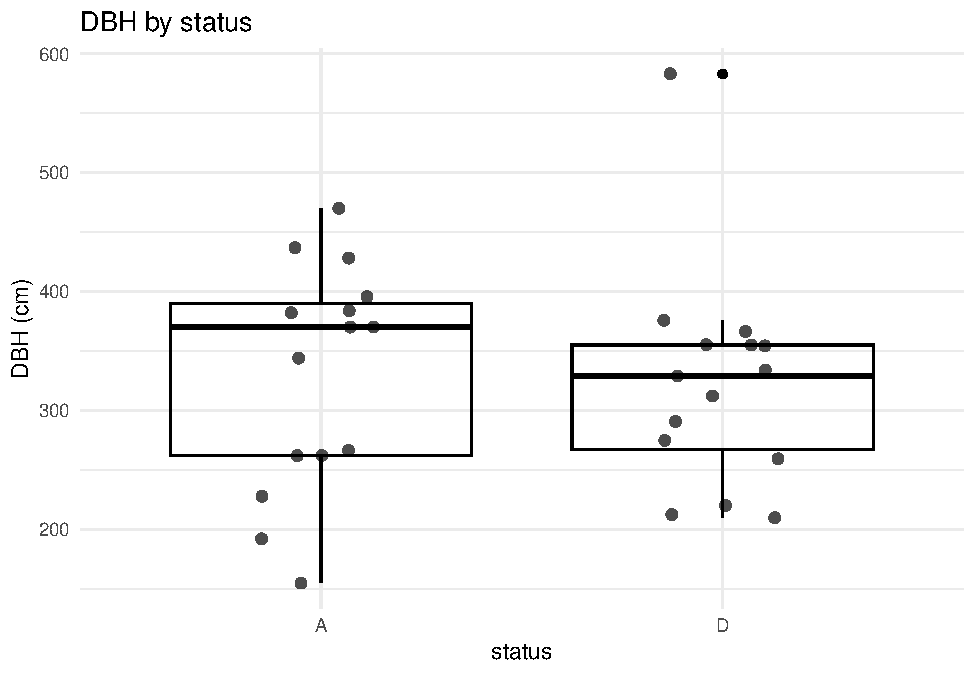
\includegraphics[keepaspectratio]{actividad2_4_files/figure-latex/unnamed-chunk-2-1.pdf}}

\section{Site map}\label{site-map}

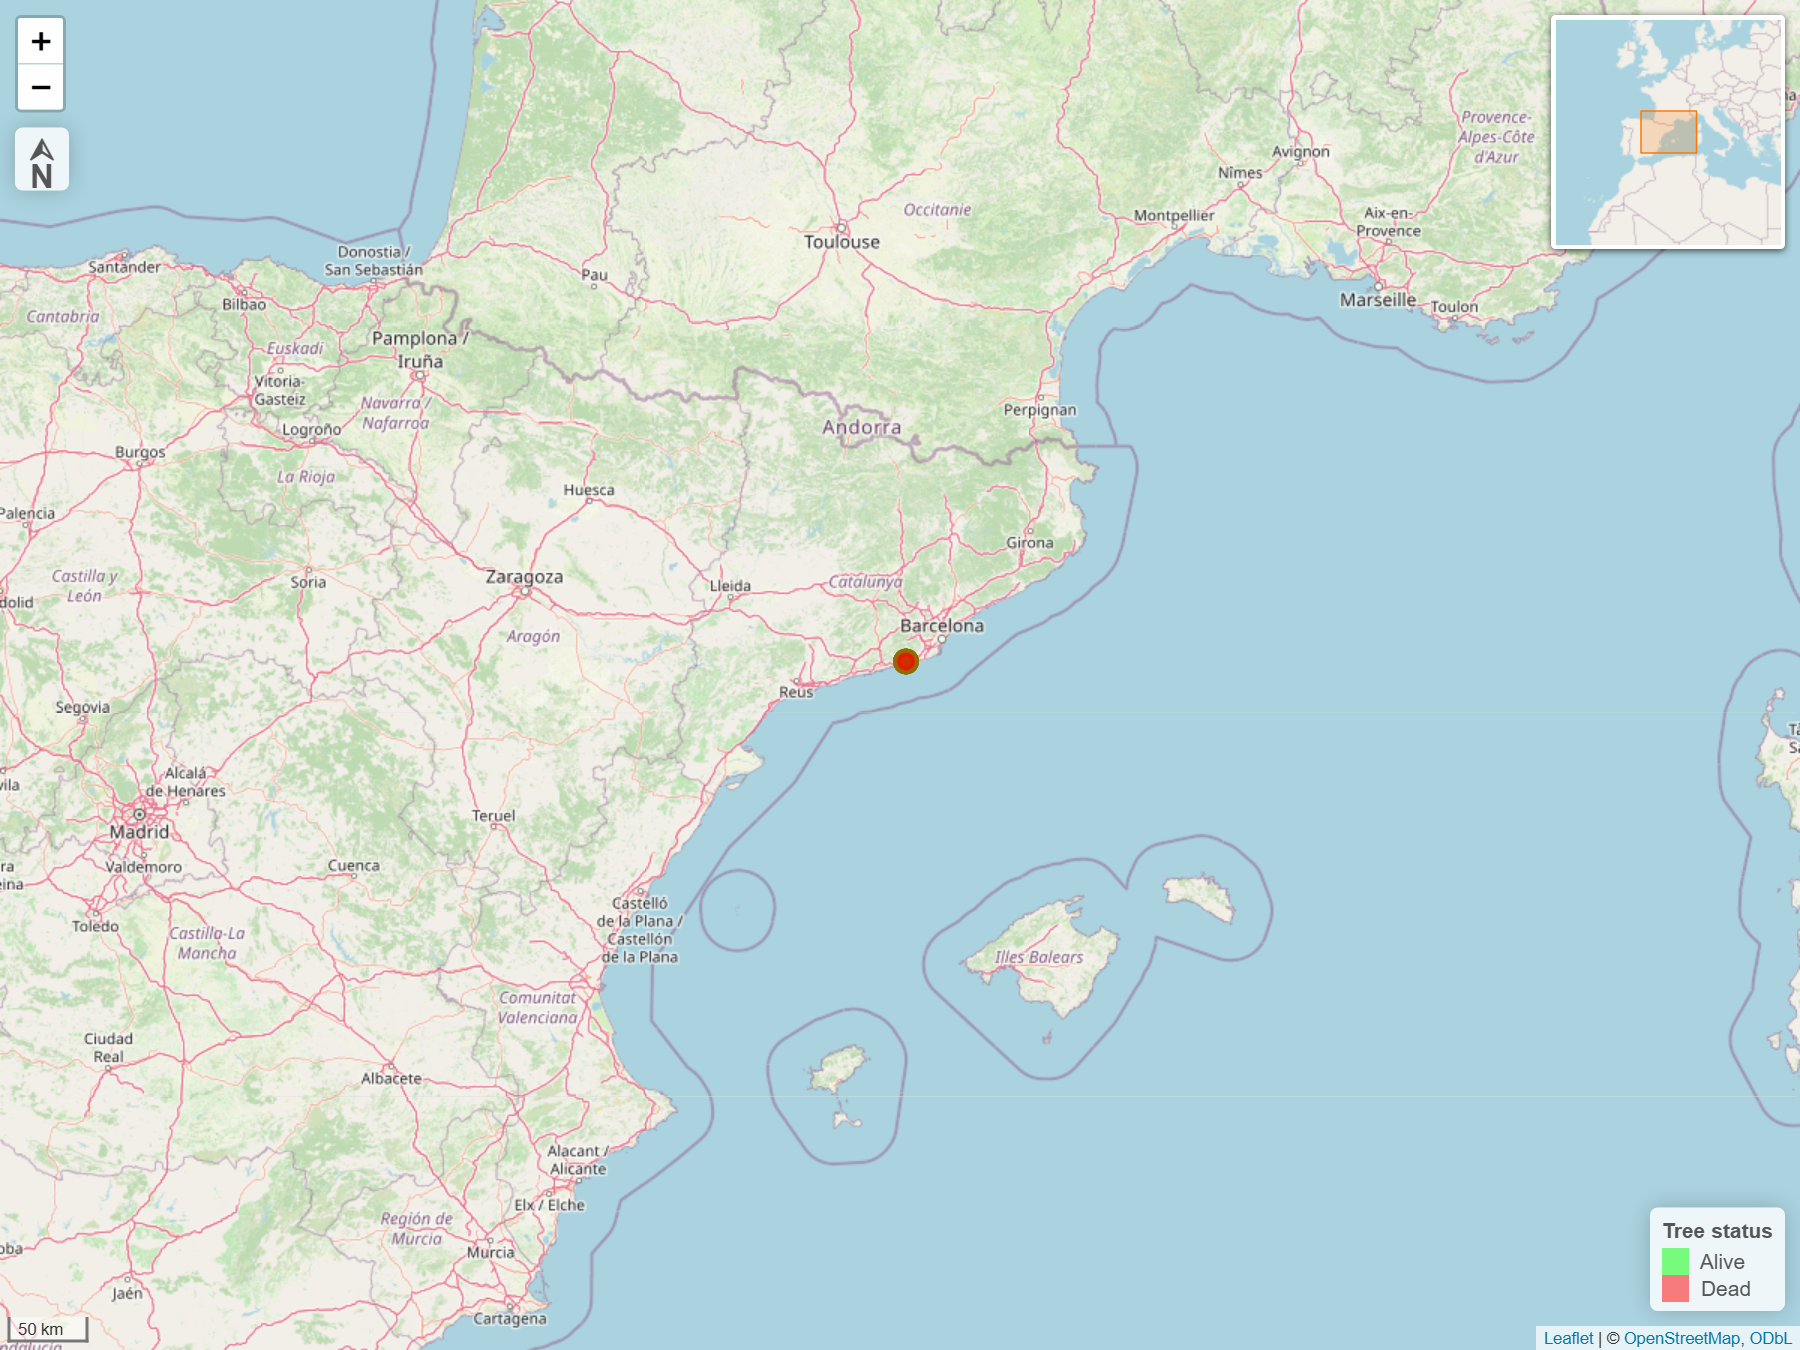
\includegraphics[width=1\linewidth]{mapa_arbre}

\newpage

\subsection*{Bibliography}\label{bibliography}
\addcontentsline{toc}{subsection}{Bibliography}

\phantomsection\label{refs}
\begin{CSLReferences}{1}{0}
\bibitem[\citeproctext]{ref-coughlandeperez2022}
Coughlan de Perez, E., Harrison, L., Berse, K., Easton-Calabria, E.,
Marunye, J., Marake, M., Murshed, S. B., Shampa, \& Zauisomue, E.-H.
(2022). Adapting to climate change through anticipatory action: The
potential use of weather-based early warnings. \emph{Weather and Climate
Extremes}, \emph{38}, 100508.
\url{https://doi.org/10.1016/j.wace.2022.100508}

\bibitem[\citeproctext]{ref-lemus-canovas2024}
Lemus-Canovas, M., Insua-Costa, D., Trigo, R. M., \& Miralles, D. G.
(2024). Record-shattering 2023 Spring heatwave in western Mediterranean
amplified by long-term drought. \emph{Npj Climate and Atmospheric
Science}, \emph{7}(1), 25.
\url{https://doi.org/10.1038/s41612-024-00569-6}

\bibitem[\citeproctext]{ref-prohom2023}
Prohom, M., Domonkos, P., Cunillera, J., Barrera-Escoda, A., Busto, M.,
Herrero-Anaya, M., Aparicio, A., \& Reynés, J. (2023). CADTEP : A new
daily quality{-}controlled and homogenized climate database for
Catalonia (1950{\textendash}2021). \emph{International Journal of
Climatology}, \emph{43}(11), 4771--4789.
\url{https://doi.org/10.1002/joc.8116}

\end{CSLReferences}

\end{document}
